\documentclass{article}

\usepackage[spanish]{babel}
\usepackage[numbers,sort&compress]{natbib}
\usepackage{graphicx}
\usepackage{url}
\usepackage{amsmath}
\usepackage{hyperref}
\usepackage{listings}
\usepackage[top=30mm, bottom=40mm, left=15mm, right=15mm]{geometry}
\usepackage{color}
\usepackage{subfig}
 
\definecolor{codegreen}{rgb}{0,0.6,0}
\definecolor{codegray}{rgb}{0.5,0.5,0.5}
\definecolor{codepurple}{rgb}{0.58,0,0.82}
\definecolor{backcolour}{rgb}{1,1,1}
 
\lstdefinestyle{mystyle}{
    backgroundcolor=\color{backcolour},   
    commentstyle=\color{codegreen},
    keywordstyle=\color{magenta},
    numberstyle=\tiny\color{codegray},
    stringstyle=\color{codepurple},
    basicstyle=\footnotesize,
    breakatwhitespace=false,         
    breaklines=true,                 
    captionpos=b,                    
    keepspaces=true,                 
    numbers=left,                    
    numbersep=5pt,                  
    showspaces=false,                
    showstringspaces=false,
    showtabs=false,                  
    tabsize=2
}
 
\lstset{style=mystyle}

\setlength{\parskip}{2mm}
\setlength{\parindent}{0pt}

\author{Edson Raúl Cepeda Márquez}
\title{Movimiento Browniano}
\date{\today}



\begin{document}

\maketitle

\section{Objetivo}

En esta práctica se pretende analizar el comportamiento que exhibe una partícula que realiza un Movimiento Browniano, es decir, que cambia su posición uniformemente al azar. El movimiento de dicha partícula se realizará en pasos unitarios, además,  para fines de esta práctica se moverá en 8 dimensiones.

La tarea es interpretar los datos de la simulación para comprobar si la dimensión o el número de pasos de la caminata que hace la partícula afecta o no, en la probabilidad de regreso al origen en cada una de las dimensiones. Este experimento se repetirá 30 veces, variando el número de dimensiones de uno en uno hasta llegar a 8, el número de pasos de la caminata será en potencias de dos variando el exponente de uno en uno desde una potencia de 6 hasta una potencia de 12, esto dando un mínimo de 64 pasos y un máximo de 4,096 pasos, todo esto al finalizar las iteraciones correspondientes a las 8 dimensiones.

Para la realización de la practica se hizo uso del código proporcionado \cite{satu} por nuestra profesora, este escrito en el lenguaje de programación R \cite{r}.

También se consulto el material de apoyo de su página web \cite{satu} donde viene en detalle el tema de la práctica, así como ejemplos \cite{ast,yes} que fueron útiles para la realización de este reporte. 

\section{Desarrollo}


Uno de los primeros pasos fue la interpretación y el estudio de los códigos de ejemplo, posteriormente se propuso la siguiente hipótesis antes de comenzar con la experimentación : 

Dado que la partícula deberá coincidir en el punto inicial de cada una de sus dimensiones, la probabilidad de regreso al origen decrece conforme el número de pasos aumenta, puesto que los pasos de la partícula se suman o se restan dependiendo de las probabilidades de un numero pseudoaleatorio , la partícula tendrá mas probabilidades de regresar al origen cuando solo realiza 64 pasos ($2^6$) que cuando realiza 4,096 pasos ($2^{12}$), se puede decir que la distancia que puede recorrer la partícula afecta a estas probabilidades.

Respecto a las dimensiones, la partícula tendrá mucha más libertad de movimiento si se mueve en dimensiones mayores a 3, esto provoca que sea difícil para la partícula realizar un recorrido inverso que lo lleve devuelta al origen.

Partimos de esta hipótesis para guiarnos sobre lo que debemos comprobar. Empecemos por comprobar si la distancia afecta o no.

Para medir la distancia máxima que alcanza cada partícula podemos usar dos métodos para su cálculo, estos son la distancia Manhattan y la distancia Euclidiana, pero para obtener una mejor precisión usaremos la primera opción pues este método se asemeja más a la realidad. 

\begin{figure}
\centering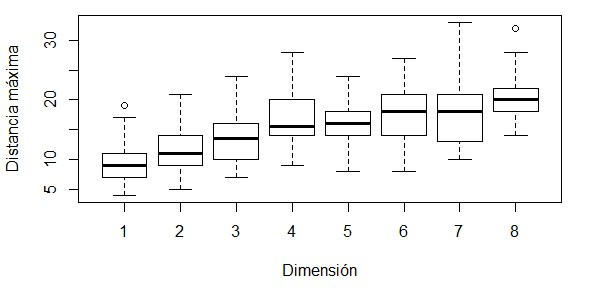
\includegraphics[width=70mm]{Distancia26.jpg}
\caption{Grafica de distancia maxima (64 pasos)}
\label{Grafica 1}
\end{figure}

\begin{figure}
\centering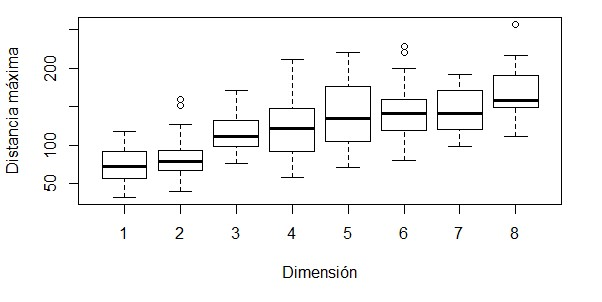
\includegraphics[width=70mm]{Distancia212.jpg}
\caption{Grafica de distancia maxima (4,096 pasos)}
\label{Grafica 2}
\end{figure}

Ahora que se pueden visualizar los resultados es posible hacer una comparación en cuanto como afecta el número de pasos en la distancia, era de intuir que a mayor número de pasos mayor probabilidad tenía la partícula de desplazarse.

Podemos observar que la primera grafica \ref{Grafica 1} la cual avanzó 64 pasos tiene un valor ligeramente arriba de 30 como distancia máxima mientras que al aumentar el número de pasos a 4,096 \ref{Grafica 2} vemos como incrementan considerablemente los valores de la distancia máxima en cada una de las dimensiones llegando a rebasar ligeramente arriba del 200.

De esta manera podemos comprobar que sí, mientras aumente el número de pasos más distancia recorres lo cual aumenta la probabilidad de que la partícula se aleje cada vez más los puntos de origen.

Ahora modificamos el código y calculamos las probabilidades de que la partícula vuelva al origen.

\lstinputlisting[language= R,firstline=1, lastline=39]{P1.R}

En el código se agregó un contador y se comprueba cuando la partícula haya cruzado por los puntos de origen, dentro de la iteración que contempla la duración (pasos) de la caminata se incluye el nuevo contador y la condición mencionada anterior mente, el valor se que se devuelve se calcula: 

\begin{equation}
P\approx \frac{N}{T}(100)
\end{equation}

En donde $P$ es la probabilidad de regreso al origen, $N$ es el numero de veces que la partícula pasa por los puntos iniciales (origen) y $T$ es el número de pasos. Multiplicado por 100 nos estaría dando el porcentaje de veces que una partícula puede regresar al origen en un determinado número de pasos.
El resultado graficado \ref{G}:

\begin{figure}[h]
\centering
\subfloat[De 64 a 2,028 pasos]{\label{f: Grafica 3}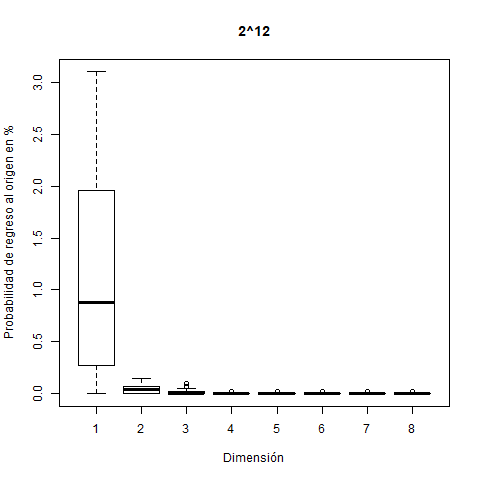
\includegraphics[width=70mm]{2e12.jpg}}
\subfloat[4,096 pasos]{\label{f: Grafica 4}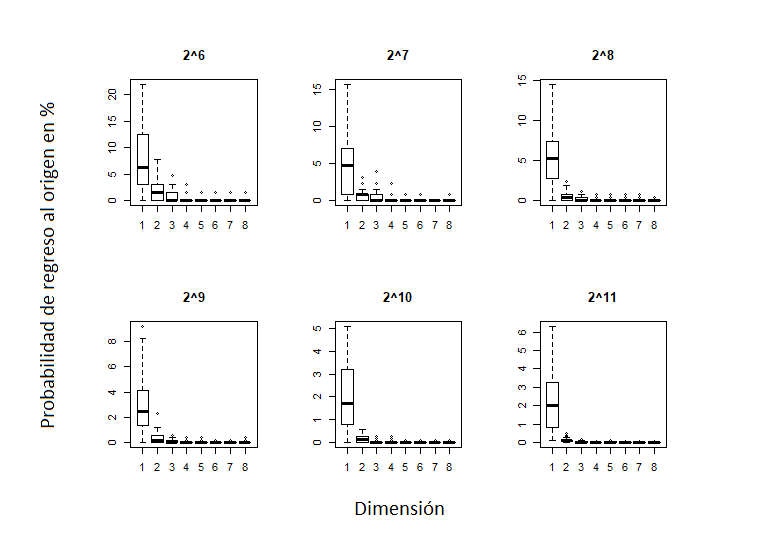
\includegraphics[width=100mm]{Probabilidades3x3.png}}
\caption{Grafica de probabilidades de regreso al origen}
\label{G}
\end{figure}

Se puede observar que las probabilidades de que la particula regrese al origen decrecen al incrementar el numero de pasos y a su vez también decrece conforme la dimensión es mayor \ref{G}. El caso más drástico fue cuando el numero de pasos era 4096 pues las probabilidades decayeron mucho incluso en la primera dimensión.

\section{Conclusiones}

Analizando la información antes presentada podemos afirmar que ambas variables, la dimensión y el numero de pasos afectan directamente a la probabilidad de que la partícula regrese al origen y éste se explica a que en cada iteración que pasa por la dimensión y o el número de pasos se aleja  más de sus puntos iniciales, es por eso que a más dimensiones mas se expande su distancia hacia y debido a su cantidad hace menos probable que la cantidad de pasos que ya dio en una dimensión se reduzca hasta llegar a 0, su punto inicial.

Aunque el efecto que tiene el número de pasos no es tan grande como el efecto que tiene las dimensiones, la reducción de posibilidades a causa de que la cantidad de iteraciones sea más larga seguirá estando presente sobre todo si el numero de pasos crece de manera exponencial.

Una buena interrogante a este problema es de ir a extremo a extremo, muchas cantidades de datos e iteraciones y muchas dimensiones para ver cómo se comporta el sistema.

Se concluye que ambas variables  ,las dimension y la duración afectan en las caminatas de una partícula con movimiento browniano y la probabilidad de regreso al origen decrece cuando estas dos cantidades aumentan.

\medskip

\begin{thebibliography}{9}

\bibitem{r} 
R:  R Project, 2019
\\\texttt{https://www.r-project.org/}

\bibitem{satu} 
Elisa Schaeffer Satu: R paralelo: simulación y análisis de datos, 2019
\\\texttt{https://elisa.dyndns-web.com/teaching/comp/par/index.html}
 

\bibitem{ast} 
Astrid Gonzales: Movimiento Browniano, 2018
\\\texttt{https://sourceforge.net/p/gla-sim/exercises/HEAD/tree/}


\bibitem{yes} 
Yessica Reyna Fernández: Practica 1 Movimiento Browniano, 2018
\\\texttt{https://sourceforge.net/projects/simulacion-de-sistemas/}

\end{thebibliography}



\end{document}